\fancyhead[L]{\textsf{\textbf{MỤC 1.4}}\quad Hàm số mũ}
\fancyhead[R]{\textsf{\textbf{51}}}

\noindent
\begin{minipage}[t]{0.26\textwidth}
    \vspace*{3.8cm}
    \noindent
    \textbf{\textsf{HÌNH 15}}\\
    {\small Đồ thị của $y = e^x$ nằm giữa các đồ thị của $y = 2^x$ và $y = 3^x$.}
\end{minipage}%
\hfill
\begin{minipage}[t]{0.71\textwidth}
    \noindent
    Từ các Hình 12 và 13, không có gì đáng ngạc nhiên khi số $e$ nằm giữa 2 và 3 và đồ thị của $y = e^x$ nằm giữa các đồ thị của $y = 2^x$ và $y = 3^x$. (Xem Hình 15.) Trong Chương 3, chúng ta sẽ thấy rằng giá trị của $e$, chính xác đến năm chữ số thập phân, là
    \[
    e \approx 2{,}71828
    \]
    Chúng ta gọi hàm số $f(x) = e^x$ là \textbf{hàm số mũ tự nhiên}.

    \begin{center}
        \vspace{-2pt}
        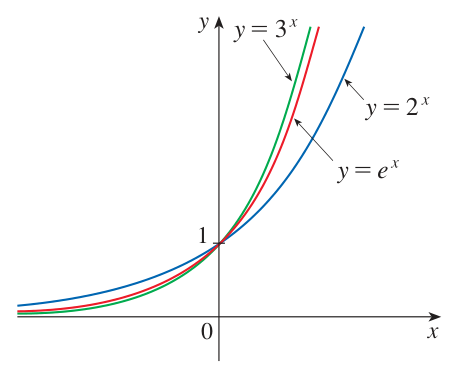
\includegraphics[width=0.52\linewidth]{images/p0086_fig1.png}
        \vspace{-2pt}
    \end{center}

    \noindent
    \textbf{\textsf{\color{stewartcyan}VÍ DỤ 5}}\hspace{0.8em}Vẽ đồ thị hàm số $y = \frac{1}{2}e^{-x} - 1$ và xác định tập xác định cùng tập giá trị của nó.

    \vspace{0.15cm}
    \noindent
    \textbf{\textsf{\color{stewartcyan}LỜI GIẢI}}\hspace{0.8em}Ta bắt đầu với đồ thị của $y = e^x$ từ các Hình 14 và 16(a), rồi lấy đối xứng qua trục $y$ để thu được đồ thị của $y = e^{-x}$ trong Hình 16(b). (Lưu ý rằng tiếp tuyến của đồ thị tại giao điểm với trục $y$ có hệ số góc bằng $-1$.) Sau đó, ta co đồ thị theo phương thẳng đứng với hệ số 2 để nhận được đồ thị của $y = \frac{1}{2}e^{-x}$ trong Hình 16(c). Cuối cùng, ta tịnh tiến đồ thị xuống dưới một đơn vị để thu được đồ thị mong muốn trong Hình 16(d). Tập xác định là $\mathbb{R}$ và tập giá trị là $(-1, \infty)$.
\end{minipage}

\vspace{0.35cm}
\noindent
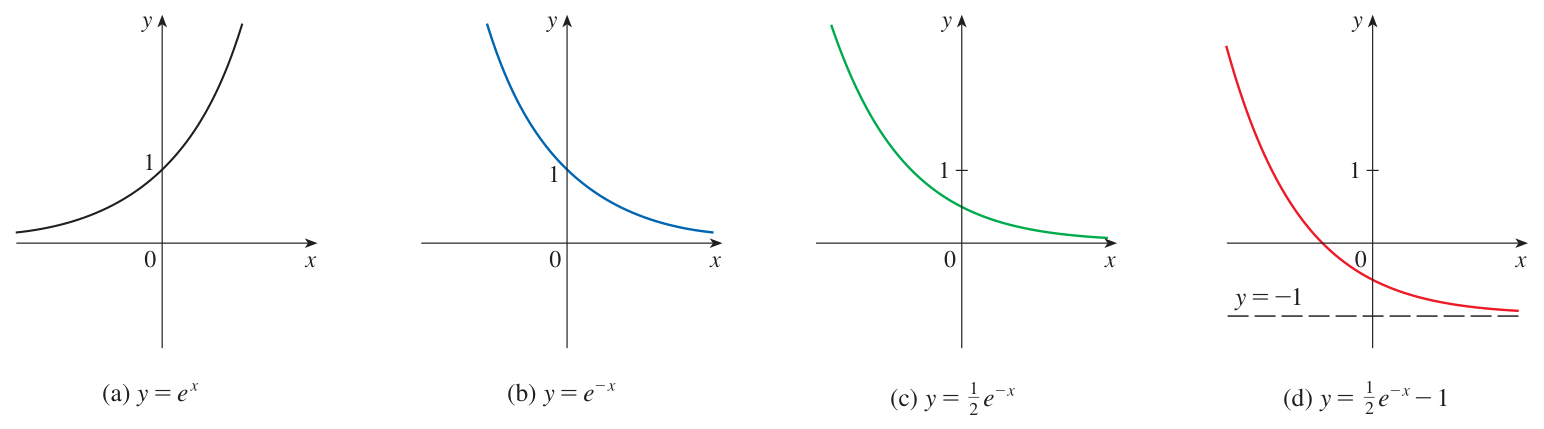
\includegraphics[width=\textwidth]{images/p0086_fig2.png}\par\vspace{4pt}
\noindent
\textbf{\textsf{HÌNH 16}}\hfill{\color{stewartcyan}$\blacksquare$}

\vspace{0.35cm}
\noindent
\begin{minipage}[t]{0.26\textwidth}
    \vspace*{0.25cm}
    \noindent
    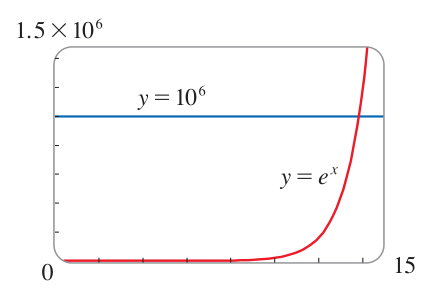
\includegraphics[width=\linewidth]{images/p0086_fig3.png}\par\vspace{4pt}
    \textbf{\textsf{HÌNH 17}}
\end{minipage}%
\hfill
\begin{minipage}[t]{0.71\textwidth}
    \noindent
    Bạn nghĩ chúng ta sẽ phải đi xa bao nhiêu về phía bên phải để độ cao của đồ thị hàm số $y = e^x$ vượt quá một triệu? Ví dụ sau đây minh họa tốc độ tăng trưởng nhanh chóng của hàm số này bằng cách đưa ra một câu trả lời có thể khiến bạn bất ngờ.

    \vspace{0.25cm}
    \noindent
    \textbf{\textsf{\color{stewartcyan}VÍ DỤ 6}}\hspace{0.8em}Sử dụng máy tính cầm tay có chức năng vẽ đồ thị hoặc máy tính để tìm các giá trị của $x$ sao cho $e^x > 1\,000\,000$.

    \vspace{0.15cm}
    \noindent
    \textbf{\textsf{\color{stewartcyan}LỜI GIẢI}}\hspace{0.8em}Trong Hình 17, chúng ta vẽ đồ thị của cả hàm số $y = e^x$ và đường thẳng nằm ngang $y = 1\,000\,000$. Ta thấy rằng hai đường cong này giao nhau khi $x \approx 13{,}8$. Do đó $e^x > 10^6$ khi $x > 13{,}8$. Có lẽ điều gây ngạc nhiên là giá trị của hàm số mũ đã vượt ngưỡng một triệu khi $x$ mới chỉ bằng 14.\hfill{\color{stewartcyan}$\blacksquare$}
\end{minipage}